\section{Experiments}
\label{sec:experiments}

\begin{figure}[t]
    \vspace*{-2px}
    \centering
    
    \begin{minipage}[t]{0.225\textwidth}
        \vspace*{0px}
        
        \centering
        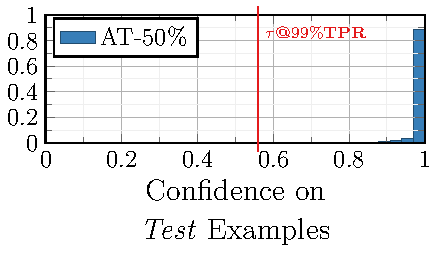
\includegraphics[width=1\textwidth]{fig_msvhn_corr_advtrain}
        \vspace*{-14px}
        
        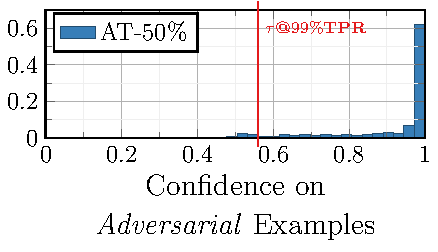
\includegraphics[width=1\textwidth]{fig_msvhn_succ_advtrain}
    \end{minipage}
    \begin{minipage}[t]{0.225\textwidth}
        \vspace*{0px}
        
        \centering
        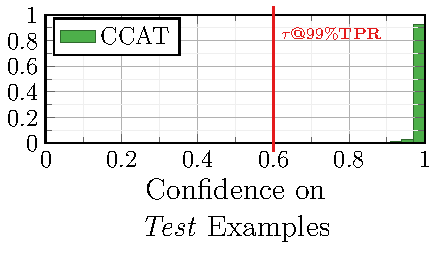
\includegraphics[width=1\textwidth]{fig_msvhn_corr_ours10}
        \vspace*{-14px}
        
        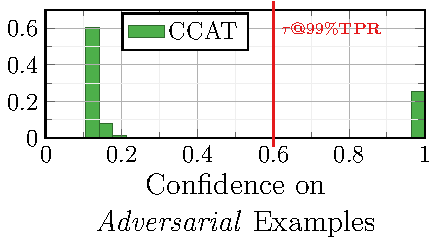
\includegraphics[width=1\textwidth]{fig_msvhn_succ_ours10}
    \end{minipage}
    
    \vspace*{-8px}
    \caption{\textbf{Confidence Histograms.} On SVHN, for \AdvTrain ($50\%$/$50\%$ adversarial training, left) and \ConfTrain (right), we show confidence histograms corresponding to \emph{correctly classified} test examples (top) and adversarial examples (bottom). We consider the worst-case adversarial examples across all $L_\infty$ attacks for $\epsilon = 0.03$. While the confidence of adversarial examples is reduced slightly for \AdvTrain, \ConfTrain is able to distinguish the majority of adversarial examples from (clean) test examples by confidence thresholding (in \textcolor{colorbrewer1}{red}).}
    \label{fig:experiments-histograms}
    \vspace*{-8px}
\end{figure}

We evaluate \ConfTrain in comparison with \AdvTrain \cite{MadryICLR2018} and related work \citep{MainiICML2020,ZhangICML2019} on MNIST \citep{LecunIEEE1998}, SVHN \citep{NetzerNIPS2011} and Cifar10 \citep{Krizhevsky2009} as well as MNIST-C \cite{MuICMLWORK2019} and Cifar10-C \cite{HendrycksICLR2019} with corrupted examples (\eg, blur, noise, compression, transforms \etc). We report \textbf{\textit{confidence-thresholded} test error (\TE; $\downarrow$ lower is better)} and \textbf{\textit{confidence-thresholded} robust test error (\RTE; $\downarrow$ lower is better)} for a confidence-threshold $\tau$ corresponding to $99\%$ true positive rate (TPR); we omit $\tau$ for brevity. We note that normal and standard adversarial training (\AdvTrain) are also allowed to reject examples by confidence thresholding. \TE is computed on $9000$ test examples. \RTE is computed on $1000$ test examples. The confidence threshold $\tau$ depends \emph{only} on correctly classified clean examples and is fixed at $99\%$TPR on the held-out \emph{last} $1000$ test examples.

\textbf{Attacks:}
%
For thorough evaluation, we consider $7$ different $L_p$ attacks for $p \in \{\infty, 2, 1, 0\}$. As white-box attacks, we use \PGD to maximize the objectives \eqnref{eq:attack} and \eqref{eq:conf-attack}, referred to as \PGD-\FCE and \PGD-\FConf. We use $T = 1000$ iterations and $10$ random restarts with random initialization plus one restart with zero initialization for \PGD-\FConf, and $T = 200$ with $50$ random restarts for \PGD-\FCE. For $L_\infty$, $L_2$, $L_1$ and $L_0$ attacks, we set \textbf{$\boldsymbol{\epsilon}$ to $\boldsymbol{0.3, 3, 18, 15}$ (MNIST) or $\boldsymbol{0.03, 2, 24, 10}$ (SVHN/Cifar10)}.

As black-box attacks, we additionally use the Query Limited (QL) attack \cite{IlyasICML2018} adapted with momentum and backtracking for $T = 1000$ iterations with $10$ restarts, the Simple attack \citep{NarodytskaCVPRWORK2017} for $T = 1000$ iterations and $10$ restarts, and the Square attack ($L_\infty$ and $L_2$) \citep{AndriushchenkoARXIV2019} with $T = 5000$ iterations. In the case of $L_0$ we also use Corner Search (CS) \citep{CroceICCV2019}. For all $L_p$, $p \in \{\infty, 2, 1, 0\}$, we consider $5000$ (uniform) random samples from the $L_p$-ball and the Geometry attack \cite{KhouryARXIV2018}. Except for CS, all black-box attacks use \eqnref{eq:conf-attack} as objective:

{\footnotesize
\vskip -2px
\begin{tabular}{| l | l | c | c |}
	\hline
	Attack & Objective & $T$ & Restarts\\\hline\hline
	\PGD-\FCE & \eqnref{eq:attack}, random init. & 200 & 50\\
	\PGD-\FConf & \eqnref{eq:conf-attack}, zero + random init. & 1000 & 11\\
	QL$^{\boldsymbol{\dagger}}$ & \eqnref{eq:conf-attack}, zero + random init. & 1000 & 11\\
	Simple$^{\boldsymbol{\dagger}}$ & \eqnref{eq:conf-attack} & 1000 & 10\\
	Square$^{\boldsymbol{\dagger}}$ & \eqnref{eq:conf-attack}, $L_\infty$, $L_2$ only & 5000 & 1\\
	CS$^{\boldsymbol{\dagger}}$ & \eqnref{eq:attack}, $L_0$ only & 200 & 1\\
	Geometry$^{\boldsymbol{\dagger}}$ & \eqnref{eq:conf-attack} & 1000 & 1\\
	Random$^{\boldsymbol{\dagger}}$ & \eqnref{eq:conf-attack} & -- & 5000\\
	\hline
    \multicolumn{4}{l}{\scriptsize $\boldsymbol{\dagger}$ Black-box attacks.}
\end{tabular}
\vskip -2px
}

Additionally, we consider adversarial frames and distal adversarial examples: Adversarial frames \cite{ZajaxAAAIWORK2019} allow a $2$ (MNIST) or $3$ (SVHN/Cifar10) pixel border to be manipulated arbitrarily within $[0,1]$ to maximize \eqnref{eq:conf-attack} using \PGD. Distal adversarial examples start with a (uniform) random image and use \PGD to maximize \eqref{eq:conf-attack} within a $L_\infty$-ball of size $\epsilon = 0.3$ (MNIST) or $\epsilon = 0.03$ (SVHN/Cifar10).

\begin{table}[t]
    \centering
    \footnotesize
    \begin{tabularx}{0.45\textwidth}{| X |c|c|c|c|c|c|}
    \hline
    & \multicolumn{6}{c |}{\textbf{SVHN:} \RTE@$99\%$TPR, $L_\infty$, $\epsilon = 0.03$}\\
    \hline
    & \begin{tabular}{@{}c@{}}worst\\case\end{tabular} & \multicolumn{5}{c |}{\begin{tabular}{@{}c@{}}top-$5$ attacks/restarts\\out of $7$ attacks with $84$ restarts\end{tabular}}\\
    \hline
    \hline
    \AdvTrainHalf & 56.0 & 52.1 & 52.0 & 51.9 & 51.6 & 51.4\\
    \ConfTrain & 39.1 & 23.6 & 13.7 & 13.6 & 12.6 & 12.5\\
    \hline
\end{tabularx}
    %\vskip -4px
    \caption{\textbf{Per-Example Worst-Case Evaluation.} We compare confidence-thresholded \RTE with $\tau$@$99\%$TPR for the per-example worst-case and the top-$5$ individual attacks/restarts among $7$ attacks with $84$ restarts in total. Multiple restarts are \emph{necessary} to effectively attack \ConfTrain, while a single attack and restart is nearly sufficient against \AdvTrainHalf. This demonstrates that \ConfTrain is more difficult to ``crack''.}
    \label{tab:experiments-per-attack}
    %\vspace*{-4px}
\end{table}

\textbf{Training:}
%
We train $50\%$/$50\%$ \AdvTrain (\AdvTrainHalf) and \ConfTrain as well as $100\%$ \AdvTrain (\AdvTrainFull) with $L_\infty$ attacks using $T = 40$ iterations for \PGD-\FCE and \PGD-\FConf, respectively, and $\epsilon = 0.3$ (MNIST) or $\epsilon = 0.03$ (SVHN/Cifar10). We use ResNet-20 \citep{HeCVPR2016}, implemented in PyTorch \citep{PaszkeNIPSWORK2017}, trained using stochastic gradient descent. For \ConfTrain, we use $\rho = 10$.

\textbf{Baselines:}
%
We compare to multi-steepest descent (\Wong) adversarial training \cite{MainiICML2020} using the pre-trained LeNet on MNIST and pre-activation ResNet-18 on Cifar10 trained with $L_\infty$, $L_2$ and $L_1$ adversarial examples and $\epsilon$ set to $0.3, 1.5, 12$ and $0.03, 0.5, 12$, respectively. The $L_2$ and $L_1$ attacks in \tabref{tab:experiments-main} (larger $\epsilon$) are unseen. For \TRADES \cite{ZhangICML2019}, we use the pre-trained convolutional network \cite{CarliniSP2017} on MNIST and WRN-10-28 \cite{ZagoruykoBMVC2016} on Cifar10, trained on $L_\infty$ adversarial examples with $\epsilon=0.3$ and $\epsilon=0.03$, respectively. On Cifar10, we further consider the pre-trained ResNet-50 of \cite{MadryICLR2018} (\MadryAT, $L_\infty$ adversarial examples with $\epsilon = 0.03$). We also consider the Mahalanobis (\Lee) \cite{LeeNIPS2018} and local intrinsic dimensionality (\Ma) detectors \cite{MaICLR2018} using the provided pre-trained ResNet-34 on SVHN/Cifar10.

\begin{figure}[t]%{0.99\textwidth}
    \vspace*{-1px}
    
    \begin{minipage}[t]{0.235\textwidth}
        \vspace*{-4px}
        
        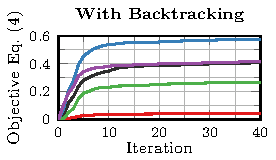
\includegraphics[width=1\textwidth]{fig_msvhn_attack_error_advtrain_0}
    \end{minipage}
    \begin{minipage}[t]{0.235\textwidth}
        \vspace*{-4px}
        
        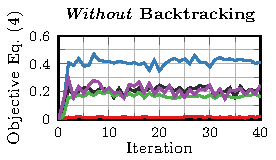
\includegraphics[width=1\textwidth]{fig_msvhn_attack_error_advtrain_2}
    \end{minipage}
    \\
    %\begin{center}
    \fbox{
        \hspace*{0.9cm}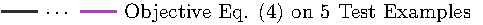
\includegraphics[width=0.35\textwidth]{fig_attack_legend}\hspace*{0.9cm}
    }
    %\end{center}
    \vspace*{-14px}
    \caption{\textbf{Backtracking.} Our $L_\infty$ \PGD-\FConf attack, \ie, \PGD maximizing \eqnref{eq:conf-attack}, using $40$ iterations with momentum and our developed backtracking scheme (left) and without both (right) on SVHN. We plot \eqnref{eq:conf-attack} over iterations for the first $5$ test examples corresponding to different colors. Backtracking avoids oscillation and obtains higher overall objective values within the same number of iterations.}
    \label{fig:experiments-momback}
    \vspace*{-4px}
\end{figure}

\subsection{Ablation Study}
\label{subsec:experiments-ablation}

\textbf{Evaluation Metrics:}
%
\figref{fig:experiments-evaluation} shows ROC curves, \ie, how well adversarial examples can be rejected by confidence. As marked in \textcolor{colorbrewer1}{red}, we are only interested in the FPR for the conservative choice of $99\%$TPR, yielding the confidence threshold $\tau$. The \RTE curves highlight how robustness is influenced by the threshold: \AdvTrain also benefits from a reject option, however, not as much as \ConfTrain which has been explicitly designed for rejecting adversarial examples.

\begin{table*}[t]
	%\centering
	\footnotesize
	\hspace*{-0.2cm}
	\begin{subfigure}{0.82\textwidth}
		\centering
		\begin{tabularx}{1\textwidth}{|X|@{\hskip 7px}c@{\hskip 7px}|@{\hskip 3px}c@{\hskip 3px}|@{\hskip 7px}c@{\hskip 7px}|@{\hskip 7px}c@{\hskip 7px}|@{\hskip 7px}c@{\hskip 7px}|@{\hskip 7px}c@{\hskip 7px}|@{\hskip 7px}c@{\hskip 7px}|@{\hskip 7px}c@{\hskip 7px}|}
\hline
%\multicolumn{9}{|c|}{\textbf{MNIST:}}\\
%\hline
\textbf{MNIST:} & \multicolumn{2}{c|@{\hskip 7px}}{\textbf{\TE} $\downarrow$ in \%} & \multicolumn{6}{@{\hskip 7px}c@{\hskip 7px}|}{\emph{confidence-thresholed} \textbf{\RTE} $\downarrow$ for $\tau$@$99\%$TPR}\\
\hline
& \begin{tabular}{@{}c@{}}(clean)\\$\tau = 0$\end{tabular}
& \begin{tabular}{@{}c@{}}(clean)\\$99\%$TPR\end{tabular}
& \begin{tabular}{@{\hskip 2.5px}c@{\hskip 2.5px}}$L_\infty$\\$\epsilon = 0.3$\end{tabular}
& \begin{tabular}{@{\hskip 2.5px}c@{\hskip 2.5px}}$L_\infty$\\$\epsilon = 0.4$\end{tabular}
& \begin{tabular}{@{}c@{}}$L_2$\\$\epsilon = 3$\end{tabular}
& \begin{tabular}{@{}c@{}}$L_1$\\$\epsilon = 18$\end{tabular}
& \begin{tabular}{@{}c@{}}$L_0$\\$\epsilon = 15$\end{tabular}
& \begin{tabular}{@{}c@{}}adv.\\frames\end{tabular}
\\\hline
& (seen)
& (seen)
& \textcolor{colorbrewer3}{seen}
& \textcolor{colorbrewer1}{\bfseries unseen}
& \textcolor{colorbrewer1}{\bfseries unseen}
& \textcolor{colorbrewer1}{\bfseries unseen}
& \textcolor{colorbrewer1}{\bfseries unseen}
& \textcolor{colorbrewer1}{\bfseries unseen}
\\\hline\hline
\Normal & 0.4 & 0.1
& 100.0 % rte@99
& 100.0 % rte@99
& 100.0 % rte@99
& 100.0 % rte@99
& 92.3 % rte@99
& 87.7 % rte@99
\\
%\hline
\AdvTrainHalf & 0.5 & \bfseries 0.0
& \bfseries 1.7 % rte@99
& 100.0 % rte@99
& 81.5 % rte@99
& 24.6 % rte@99
& 23.9 % rte@99
& 73.7 % rte@99
\\
%\hline
\AdvTrainFull & 0.5 & \bfseries 0.0
& \bfseries 1.7 % rte@99
& 100.0 % rte@99
& 84.8 % rte@99
& 21.3 % rte@99
& \bfseries 13.9 % rte@99
& 62.3 % rte@99
\\
%\hline
\ConfTrain & \bfseries 0.3 & 0.1
& 7.4 % rte@99
& \bfseries 11.9 % rte@99
& \bfseries 0.3 % rte@99
& \bfseries 1.8 % rte@99
& 14.8 % rte@99
& \bfseries 0.2 % rte@99
\\
\hline\hline
\textbf{*} \Wong & 1.8 & 0.9
& 34.3 % rte@99
& 98.9 % rte@99
& 59.2 % rte@99
& 55.9 % rte@99
& 66.4 % rte@99
& 8.8 % rte@99
\\
%\hline
\textbf{*} \TRADES & 0.5 & 0.1
& 4.0 % rte@99
& 99.9 % rte@99
& 44.3 % rte@99
& 9.0 % rte@99
& 35.5 % rte@99
& \bfseries 0.2 % rte@99
\\
\hline
\end{tabularx}
	\end{subfigure}
	\begin{subfigure}{0.085\textwidth}
		\centering
		\begin{tabular}{|@{\hskip 7px}c@{\hskip 7px}|}
%\hline
%\\
\hline
\textbf{FPR} $\downarrow$\\
\hline
\begin{tabular}{@{}c@{}}distal\\\vphantom{t}\end{tabular}\\
\hline
\textcolor{colorbrewer1}{\bfseries unseen}\\
\hline
\hline
100.0 % \Normal fpr@99
\\%\hline
100.0 % \AdvTrain fpr@99
\\%\hline
100.0 % \AdvTrainFull fpr@99
\\%\hline
\bfseries 0.0 % \ConfTrain fpr@99
\\\hline\hline
100.0 % \Wong fpr@99
\\%\hline
100.0 % \TRADES fpr@99
\\\hline
\end{tabular}

	\end{subfigure}
	\begin{subfigure}{0.08\textwidth}
		\centering
		\begin{tabular}{|c|}
%\hline
%\\
\hline
\textbf{\TE} $\downarrow$\\
\hline
\begin{tabular}{@{}c@{}}corrupted\\{MNIST-C}\end{tabular}\\
\hline
\textcolor{colorbrewer1}{\bfseries unseen}\\
\hline
\hline
32.8\\ % \Normal 99
12.6\\ % \AdvTrain 99
17.6\\ % \AdvTrainFull 99
\bfseries 5.7\\ % \ConfTrain 99
\hline\hline
6.0\\ % \Wong 99
7.9\\ % \TRADES 99
\hline
\end{tabular}

	\end{subfigure}
	\vskip 2px
	\hspace*{-0.2cm}
	\begin{subfigure}[t]{0.82\textwidth}
		\centering
		\vspace*{0px}
		
		\begin{tabularx}{1\textwidth}{|X|@{\hskip 7px}c@{\hskip 7px}|@{\hskip 3px}c@{\hskip 3px}|@{\hskip 7px}c@{\hskip 7px}|@{\hskip 7px}c@{\hskip 7px}|@{\hskip 7px}c@{\hskip 7px}|@{\hskip 7px}c@{\hskip 7px}|@{\hskip 7px}c@{\hskip 7px}|@{\hskip 7px}c@{\hskip 7px}|}
\hline
%\multicolumn{9}{|c|}{\textbf{SVHN:}}\\
%\hline
\textbf{SVHN:} & \multicolumn{2}{c|@{\hskip 7px}}{\textbf{\TE} $\downarrow$ in \%} & \multicolumn{6}{@{\hskip 7px}c@{\hskip 7px}|}{\emph{confidence-thresholed} \textbf{\RTE} $\downarrow$ for $\tau$@$99\%$TPR}\\
\hline
& \begin{tabular}{@{}c@{}}(clean)\\$\tau = 0$\end{tabular}
& \begin{tabular}{@{}c@{}}(clean)\\$99\%$TPR\end{tabular}
& \begin{tabular}{@{}c@{}}$L_\infty$\\$\epsilon = 0.03$\end{tabular}
& \begin{tabular}{@{}c@{}}$L_\infty$\\$\epsilon = 0.06$\end{tabular}
& \begin{tabular}{@{}c@{}}$L_2$\\$\epsilon = 2$\end{tabular}
& \begin{tabular}{@{}c@{}}$L_1$\\$\epsilon = 24$\end{tabular}
& \begin{tabular}{@{}c@{}}$L_0$\\$\epsilon = 10$\end{tabular}
& \begin{tabular}{@{}c@{}}adv.\\frames\end{tabular}
\\\hline
& (seen)
& (seen)
& \textcolor{colorbrewer3}{seen}
& \textcolor{colorbrewer1}{\bfseries unseen}
& \textcolor{colorbrewer1}{\bfseries unseen}
& \textcolor{colorbrewer1}{\bfseries unseen}
& \textcolor{colorbrewer1}{\bfseries unseen}
& \textcolor{colorbrewer1}{\bfseries unseen}
\\\hline\hline
\Normal & 3.6 & 2.6
& 99.9 % rte@99
& 100.0 % rte@99
& 100.0 % rte@99
& 100.0 % rte@99
& 83.7 % rte@99
& 78.7 % rte@99
\\
%\hline
\AdvTrainHalf & 3.4 & 2.5
& 56.0 % rte@99
& 88.4 % rte@99
& 99.4 % rte@99
& 99.5 % rte@99
& 73.6 % rte@99
& 33.6 % rte@99
\\
%\hline
\AdvTrainFull & 5.9 & 4.6
& 48.3 % rte@99
& 87.1 % rte@99
& 99.5 % rte@99
& 99.8 % rte@99
& 89.4 % rte@99
& 26.0 % rte@99
\\
%\hline
\ConfTrain & \bfseries 2.9 & \bfseries 2.1
& \bfseries 39.1 % rte@99
& \bfseries 53.1 % rte@99
& \bfseries 29.0 % rte@99
& \bfseries 31.7 % rte@99
& \bfseries 3.5 % rte@99
& \bfseries 3.7 % rte@99
\\
\hline\hline
\textbf{*} \Ma & 3.3 & 2.2
& 91.0
& 93.1
& 92.2
& 90.0
& 41.6
& 89.8
\\
\textbf{*} \Lee & 3.3 & 2.2
& 73.0
& 79.5
& 78.1
& 67.5
& 41.5
& 9.9
\\\hline
\end{tabularx}
	\end{subfigure}
	\begin{subfigure}[t]{0.08\textwidth}
		\centering
		\vspace*{0px}
		
		\begin{tabular}{|@{\hskip 7px}c@{\hskip 7px}|}
%\hline
%\\
\hline
\textbf{FPR} $\downarrow$\\
\hline
\begin{tabular}{@{}c@{}}distal\\\vphantom{t}\end{tabular}\\
\hline
\textcolor{colorbrewer1}{\bfseries unseen}\\
\hline
\hline
87.1 % \Normal fpr@98
\\%\hline
86.3 % \AdvTrain fpr@98
\\%\hline
81.0 % \AdvTrainFull fpr@98
\\%\hline
\bfseries 0.0 % \ConfTrain fpr@98
\\\hline\hline
8.6\\
\bfseries 0.0\\
\hline
\end{tabular}

	\end{subfigure}
	\hfill
	\vskip 2px
	\hspace*{-0.2cm}
	\begin{subfigure}[t]{0.82\textwidth}
		\centering
		\vspace*{0px}
		
		\begin{tabularx}{1\textwidth}{|X|@{\hskip 7px}c@{\hskip 7px}|@{\hskip 3px}c@{\hskip 3px}|@{\hskip 7px}c@{\hskip 7px}|@{\hskip 7px}c@{\hskip 7px}|@{\hskip 7px}c@{\hskip 7px}|@{\hskip 7px}c@{\hskip 7px}|@{\hskip 7px}c@{\hskip 7px}|@{\hskip 7px}c@{\hskip 7px}|}
%\hline
%\multicolumn{9}{|c|}{\textbf{CIFAR10:}}\\
\hline
\textbf{CIFAR10:} & \multicolumn{2}{c|@{\hskip 7px}}{\textbf{\TE} $\downarrow$ in \%} & \multicolumn{6}{@{\hskip 7px}c@{\hskip 7px}|}{\emph{confidence-thresholed} \textbf{\RTE} $\downarrow$ for $\tau$@$99\%$TPR}\\
\hline
& \begin{tabular}{@{}c@{}}(clean)\\$\tau = 0$\end{tabular}
& \begin{tabular}{@{}c@{}}(clean)\\$99\%$TPR\end{tabular}
& \begin{tabular}{@{}c@{}}$L_\infty$\\$\epsilon = 0.03$\end{tabular}
& \begin{tabular}{@{}c@{}}$L_\infty$\\$\epsilon = 0.06$\end{tabular}
& \begin{tabular}{@{}c@{}}$L_2$\\$\epsilon = 2$\end{tabular}
& \begin{tabular}{@{}c@{}}$L_1$\\$\epsilon = 24$\end{tabular}
& \begin{tabular}{@{}c@{}}$L_0$\\$\epsilon = 10$\end{tabular}
& \begin{tabular}{@{}c@{}}adv.\\frames\end{tabular}
\\\hline
& (seen)
& (seen)
& \textcolor{colorbrewer3}{seen}
& \textcolor{colorbrewer1}{\bfseries unseen}
& \textcolor{colorbrewer1}{\bfseries unseen}
& \textcolor{colorbrewer1}{\bfseries unseen}
& \textcolor{colorbrewer1}{\bfseries unseen}
& \textcolor{colorbrewer1}{\bfseries unseen}
\\\hline\hline
\Normal & \underline{8.3} & 7.4
& 100.0 % rte@99
& 100.0 % rte@99
& 100.0 % rte@99
& 100.0 % rte@99
& 84.7 % rte@99
& 96.7 % rte@99
\\
%\hline
\AdvTrainHalf & 16.6 & 15.5
& 62.7 % rte@99
& 93.7 % rte@99
& 98.4 % rte@99
& 98.4 % rte@99
& 74.4 % rte@99
& 78.7 % rte@99
\\
%\hline
\AdvTrainFull & 19.4 & 18.3
& 59.9 % rte@99
& 90.3 % rte@99
& 98.3 % rte@99
& 98.0 % rte@99
& 72.3 % rte@99
& 79.6 % rte@99
\\
%\hline
\ConfTrain & 10.1 & \underline{6.7}
& 68.4 % rte@99
& 92.4 % rte@99
& \bfseries 52.2 % rte@99
& \bfseries 58.8 % rte@99
& \bfseries 23.0 % rte@99
& \bfseries 66.1 % rte@99
\\
\hline\hline
\textbf{*} \Wong & 18.4 & 17.6
& 53.2 % rte@99
& 89.4 % rte@99
& 88.5 % rte@99
& 68.6 % rte@99
& 39.2 % rte@99
& 82.6 % rte@99
\\
%\hline
\textbf{*} \TRADES & 15.2 & 13.2
& \bfseries 43.5 % rte@99
& \bfseries 81.0 % rte@99
& 70.9 % rte@99
& 96.9 % rte@99
& 36.9 % rte@99
& 72.1 % rte@99
\\
\textbf{*} \MadryAT & 13.0 & 11.7
& 45.1 % rte@99
& 84.5 % rte@99
& 98.7 % rte@99
& 97.8 % rte@99
& 42.3 % rte@99
& 73.3 % rte@99
\\
\hline\hline
\textbf{*} \Ma & \bfseries 6.4 & \bfseries 4.9
& 99.0
& 99.2
& 70.6
& 89.4
& 47.0
& \bfseries 66.1
\\
\textbf{*} \Lee & \bfseries 6.4 & \bfseries 4.9
& 94.1
& 95.3
& 90.6
& 97.6
& 49.8
& 70.0
\\\hline
\end{tabularx}
	\end{subfigure}
	\begin{subfigure}[t]{0.085\textwidth}
		\centering
		\vspace*{0px}
		
		\begin{tabular}{|@{\hskip 7px}c@{\hskip 7px}|}
%\hline
%\\
%\hline
\hline
\textbf{FPR} $\downarrow$\\
\hline
\begin{tabular}{@{}c@{}}distal\\\vphantom{t}\end{tabular}\\
\hline
\textcolor{colorbrewer1}{\bfseries unseen}\\
\hline
\hline
83.3 % \Normal fpr@99
\\%\hline
75.0 % \AdvTrain fpr@99
\\%\hline
72.5 % \AdvTrainFull fpr@99
\\%\hline
\bfseries 0.0 % \ConfTrain fpr@99
\\\hline\hline
76.7 % \Wong fpr@99
\\%\hline
76.2 % \TRADES fpr@99
\\%\hline
78.5 % \MadryAT fpr@99
\\\hline\hline
0.1\\
2.4\\
\hline
\end{tabular}

	\end{subfigure}
	\begin{subfigure}[t]{0.08\textwidth}
		\centering
		\vspace*{0px}
		
		\begin{tabular}{|@{\hskip 7px}c@{\hskip 7px}|}
%\hline
%\\
\hline
\textbf{\TE} $\downarrow$\\
\hline
\begin{tabular}{@{}c@{}}corrupted\\{\scriptsize CIFAR10-C}\end{tabular}\\
\hline
\textcolor{colorbrewer1}{\bfseries unseen}\\
\hline
\hline
12.3\\
16.2\\
19.6\\
\bfseries 8.5\\
\hline\hline
19.3\\
15.0\\
12.9\\
\hline\hline
11.59\\
12.4\\
\hline
\end{tabular}

	\end{subfigure}
	\vskip -6px
	\caption{\textbf{Main Results: Generalizing Robustness.} For $L_\infty$, $L_2$, $L_1$, $L_0$ attacks and adversarial frames, we report per-example worst-case (confidence-thresholded) \TE and \RTE at $99\%$TPR across all attacks; $\epsilon$ is reported in the corresponding columns. For distal adversarial examples and corrupted examples, we report FPR and \TE, respectively. $L_\infty$ attacks with $\epsilon{=}0.3$ on MNIST and $\epsilon = 0.03$ on SVHN/Cifar10 were used for training (\textcolor{colorbrewer3}{seen}). The remaining attacks were not encountered during training (\textbf{\textcolor{colorbrewer1}{unseen}}). \ConfTrain outperforms \AdvTrain and the other baselines regarding robustness against unseen attacks. FPRs included in the supplementary material. \textbf{*}~Pre-trained models with different architecture, \Ma/\Lee use the same model.}
	\label{tab:experiments-main}
    \vspace*{-2px}
\end{table*}

\textbf{Worst-Case Evaluation:} 
%
\tabref{tab:experiments-per-attack} illustrates the importance of worst-case evaluation on SVHN, showing that \ConfTrain is significantly ``harder'' to attack than \AdvTrain. We show the worst-case \RTE over all $L_\infty$ attacks as well as the top-$5$ individual attacks (each restart treated as separate attack). For \AdvTrainHalf, a single restart of \PGD-\FConf with $T=1000$ iterations is highly successful, with $52.1\%$ \RTE close to the overall worst-case of $56\%$. For \ConfTrain, in contrast, multiple restarts are crucial as the best individual attack, \PGD-\FConf with $T=1000$ iterations and zero initialization obtains only $23.6\%$ \RTE compared to the overall worst-case of $39.1\%$.

\textbf{Backtracking:}
%
\figref{fig:experiments-momback} illustrates the advantage of backtracking for \PGD-\FConf with $T{=}40$ iterations on $5$ test examples of SVHN. Backtracking results in better objective values and avoids oscillation, \ie, a stronger attack for training and testing. In addition, while $T{=}200$ iterations are sufficient against \AdvTrain, we needed up to $T{=}1000$ iterations for \ConfTrain.

\subsection{Main Results (Table  \ref{tab:experiments-main})}
\label{subsec:experiments-main}

\textbf{Robustness Against \textcolor{colorbrewer3}{seen} $L_\infty$ Attacks:}
%
Considering \tabref{tab:experiments-main} and $L_\infty$ adversarial examples as \textcolor{colorbrewer3}{seen} during training, \ConfTrain exhibits comparable robustness to \AdvTrain. With $7.4\%$/$67.9\%$ \RTE on MNIST/Cifar10, \ConfTrain lacks behind \AdvTrainHalf ($1.7\%$/$62.7\%$) only slightly. On SVHN, in contrast \ConfTrain outperforms \AdvTrainHalf and \AdvTrainFull significantly with $39.1\%$ vs. $56.0\%$ and $48.3\%$. We note that \ConfTrain and \AdvTrainHalf are trained on $50\%$ clean / $50\%$ adversarial examples. This is in contrast to \AdvTrainFull trained on $100\%$ adversarial examples, which improves robustness slightly, \eg, from $56\%$/$62.7\%$ to $48.3\%$/$59.9\%$ on SVHN/Cifar10.

\textbf{Robustness Against \textcolor{colorbrewer1}{unseen} $L_p$ Attacks:}
%
Regarding \textcolor{colorbrewer1}{unseen} attacks, \AdvTrain's robustness deteriorates quickly while \ConfTrain is able to generalize robustness to novel threat models. On SVHN, for example, \RTE of \AdvTrainHalf goes up to $88.4\%$, $99.4\%$, $99.5\%$ and $73.6\%$ for larger $L_\infty$, $L_2$, $L_1$ and $L_0$ attacks. In contrast, \ConfTrain's robustness generalizes to these unseen attacks significantly better, with $53.1\%$, $29\%$, $31.7\%$ and $3.5\%$, respectively. The results on MNIST and Cifar10 or for \AdvTrainFull tell a similar story. However, \AdvTrain generalizes better to $L_1$ and $L_0$ attacks on MNIST, possibly due to the large $L_\infty$-ball used during training ($\epsilon = 0.3$). Here, training purely on adversarial examples, \ie, \AdvTrainFull is beneficial. On Cifar10, \ConfTrain has more difficulties with large $L_\infty$ attacks ($\epsilon = 0.06$) with $92\%$ \RTE.
As detailed in the supplementary material, these observations are supported by considering FPR. \AdvTrain benefits from considering FPR as clean \TE is not taken into account. On Cifar10, for example, $47.6\%$ FPR compared to $62.7\%$ \RTE for \AdvTrainHalf. This is less pronounced for \ConfTrain due to the improved \TE compared to \AdvTrain. Overall, \ConfTrain improves robustness against arbitrary (unseen) $L_p$ attacks, demonstrating that \ConfTrain indeed extrapolates near-uniform predictions beyond the $L_\infty$ $\epsilon$-ball used during training.

 
\textbf{Comparison to \Wong and \TRADES:}
%
\TRADES is able to outperform \ConfTrain alongside \AdvTrain (including \MadryAT) on Cifar10 with respect to the $L_\infty$ adversarial examples \textcolor{colorbrewer3}{seen} during training: $43.5\%$ \RTE compared to $68.4\%$ for \ConfTrain. This might be a result of training on $100\%$ adversarial examples and using more complex models: \TRADES uses a WRN-10-28 with roughly $46.1\text{M}$ weighs, in contrast to our ResNet-18 with $4.3\text{M}$ (and ResNet-20 with $11.1\text{M}$ for \Wong). However, regarding \textcolor{colorbrewer1}{unseen} $L_2$, $L_1$ and $L_0$ attacks, \ConfTrain outperforms \TRADES with $52.2\%$, $58.8\%$ and $23\%$ compared to $70.9\%$, $96.9\%$ and $36.9\%$ in terms of \RTE. Similarly, \ConfTrain outperforms \Wong. This is surprising, as \Wong trains on both $L_2$ and $L_1$ attacks with smaller $\epsilon$, while \ConfTrain does not. Only against larger $L_\infty$ adversarial examples with $\epsilon = 0.06$, \TRADES reduces \RTE from $92.4\%$ (\ConfTrain) to $81\%$. Similar to \AdvTrain, \TRADES also generalizes better to $L_2$, $L_1$ or $L_0$ on MNIST, while \Wong is not able to compete. Overall, compared to \Wong and \TRADES, the robustness obtained by \ConfTrain generalizes better to previously unseen attacks. We also note that, on MNIST, \ConfTrain outperforms the robust Analysis-by-Synthesis (ABS) approach of \cite{SchottICLR2019} \wrt $L_\infty$, $L_2$, and $L_0$ attacks.

\textbf{Detection Baselines:}
%
The detection methods \Ma and \Lee are outperformed by \ConfTrain across all datasets and threat models. On SVHN, for example, \Lee obtains $73\%$ \RTE against the seen $L_\infty$ attacks and $79.5\%$, $78.1\%$, $67.5\%$ and $41.5\%$ \RTE for the unseen $L_\infty$, $L_2$, $L_1$ and $L_0$ attacks. \Ma is consistently outperformed by \Lee on SVHN. This is striking, as we \emph{only} used \PGD-\FCE and \PGD-\FConf to attack these approaches and emphasizes the importance of training \emph{adversarially} against an adaptive attack to successfully reject adversarial examples.

\textbf{Robustness Against Unconventional Attacks:}
%
Against adversarial frames, robustness of \AdvTrain reduces to $73.7\%$ /$62.3\%$ \RTE (AT-$50\%$/$100\%$), even on MNIST, while \ConfTrain achieves $0.2\%$. \Wong, in contrast, is able to preserve robustness better with $8.8\%$ \RTE, which might be due to the $L_2$ and $L_1$ attacks seen during training. \ConfTrain outperforms both approaches with $0.2\%$ \RTE, as does \TRADES. On SVHN and Cifar10, however, \ConfTrain outperforms all approaches, including \TRADES, considering adversarial frames.
Against distal adversarial examples, \ConfTrain outperforms all approaches significantly, with $0\%$ FPR, compared to the second-best of $72.5\%$ for \AdvTrainFull on Cifar10. Only the detection baselines \Ma and \Lee are competitive, reaching close to $0\%$ FPR.
This means that \ConfTrain is able to extrapolate low-confidence distributions to far-away regions of the input space.
Finally, we consider corrupted examples (\eg, blur, noise, transforms \etc) where \ConfTrain also improves results, \ie, mean \TE across all corruptions. On Cifar10-C, for example, \ConfTrain achieves $8.5\%$ compared $12.9\%$ for \MadryAT and $12.3\%$ for normal training. On MNIST-C, only \Wong yields a comparably low \TE: $6\%$ vs. $5.7\%$ for \ConfTrain.

\textbf{Improved Test Error:}
%
\ConfTrain also outperforms \AdvTrain regarding \TE, coming close to that of normal training. On all datasets, \emph{confidence-thresholded} \TE for \ConfTrain is better or equal than that of normal training. On Cifar10, only \Ma/\Lee achieve a better standard and confidence-thresholded \TE using a ResNet-34 compared to our ResNet-20 for \ConfTrain ($21.2\text{M}$ vs. $4.3\text{M}$ weights). In total the performance of \ConfTrain shows that the robustness-generalization trade-off can be improved significantly.

Our \textbf{supplementary material} includes detailed descriptions of our \PGD-\FConf attack (including pseudo-code), a discussion of our confidence-thresholded \RTE, and more details regarding baselines. We also include results for confidence thresholds at $98\%$ and $95\%$TPR, which improves results only slightly, at the cost of ``throwing away'' significantly more clean examples. Furthermore, we provide ablation studies, qualitative examples and per-attack results.
